%INSTRUCTIONS ---> Go Here https://github.com/tsgoten/modern-physics-consice
%Scroll down to the bottom; Beneath the \tableofcontents there are a bunch of commented lines
%Uncomment the relevant line for your chapter to view the file

\documentclass[11pt, letterpaper, twocolumn]{report}
%Packages
\usepackage{amsmath, amsfonts, amssymb, amsthm}
\usepackage{graphicx, physics}
%Information
\author{Shivam, Tarang, Matt, Rohil, Akshit, Danny}
\title{A Concise Review of Modern Physics }
%Theorems
\theoremstyle{definition}
\newtheorem{example}{Example}[section]
\newtheorem{problem}{Problem}[section]
\newtheorem{exercise}{}
\newtheorem{q}{}[section]
\newtheorem{ans}{}[section]
%Graphics Path
\graphicspath{{graphics/}}
%Commands
\newcommand{\dif}[2]{\frac{d#1}{d#2}}
\newcommand{\diff}[3]{\frac{d^#3 #1}{d #2^#3}}
\newcommand{\wave}{\psi (x,t)}
\newcommand{\putpic}[1]{
	\begin{figure}
	\centering
	\includegraphics[width=\columnwidth]{#1}
	\end{figure}
}
\newcommand{\scinot}[2]{
	#1 \times 10^{#2}
}
\newcommand{\scinotu}[3]{
	#1 \times 10^{#2}{\mathrm{#3}}
}

\begin{document}
    \begin{titlepage}
        \begin{center}
			\vspace*{1cm}
			\Huge
			\textbf{Modern Physics}\\
			\vspace{0.5cm}
			\LARGE
			A Collection of Notes and Problems\\
			\vspace{1.5cm}
			\textbf{Tarang Srivastava}\\
			\vfill
			\vspace{0.8cm}
			\Large
			Dr. Mesut \c{C}akir\\
			Modern Physics\\
			South Brunswick High School\\
			1 June 2019
		\end{center}
    \end{titlepage}

    \tableofcontents

    % Chapters - EDIT THIS TO VIEW YOUR FILE
    % Uncomment the line and name your file to compile
    
   	%\documentclass[10pt, twocolumn]{article}
\author{Tarang Srivastava}
\usepackage{amsmath, amsthm}
\usepackage{graphicx}
\usepackage[margin=.25in]{geometry}
\geometry{letterpaper,textwidth=7.3in,hmarginratio=1:1,	textheight=9in,vmarginratio=1:1,heightrounded}
\newcommand{\makechaptertitle}[1]{
\begin{center}
	\begin{large}
		#1
	\end{large}
	\begin{small}
		\\by Tarang Srivastava
	\end{small}
\end{center}
}
\theoremstyle{definition}
\newtheorem{q}{}
\begin{document}
		\makechaptertitle{Relativity Test}
		\begin{q}
			At what speed does a clock move if it runs at a rate which is one-half the rate of a clock at rest?
		\end{q}
		\begin{q}
			At what speed does a meter stick move if its length is observed to shrink to $ 0.5 $ m?
		\end{q}
		\begin{q}
			The average lifetime of a $ \pi $ meson in its own frame of reference is $ 26.0 $ ns. (this is its proper lifetime)
			\begin{itemize}
				\item if the $ \pi $ meson moves with speed $ 0.95 c $ with respect to the Earth, what is its lifetime as measured by an observer at rest on Earth?
				\item What is the average distance it travels before decaying as measured by an observer at rest on Earth?
			\end{itemize}
		\end{q}
		\begin{q}
			An atomic clock is placed in a jet airplane. The clock measures a time interval of $ 3600 $s when the jet moves with speed $ 500 $ m/s. How much larges a time interval does an identical clock held by an observer at rest on the ground measure?
		\end{q}
		\begin{q}
			A rod of length $ L_0 $ moves with speed $ v $ along the horizontal direction. The rod makes an angle $ \theta_0 $ with respect to the $ x' $ axis. 
			\begin{itemize}
				\item Determine the length of the rod as measured by a stationary observer.
				\item Determine the angle $ \theta $ the rod makes with the $ x $ axis.
			\end{itemize}
		\end{q}
		\begin{q}
			Relativistic Doppler Shift 
			\begin{itemize}
				\item How fast and in what direction must galaxy $ A $ be moving if an absorption line found at wavelength $ 550 $nm (green) for a stationary galaxy is shifted to $ 450 $ nm (blue) ("blue shift")?
				\item How fast and in what direction is galaxy $ B $ moving if it shows the same line shifted to $ 700 $nm (red) ("red shift")?
			\end{itemize}
		\end{q}
		\begin{q}
			A stationary observer on Earth observes spaceships $ A $ and $ B $ moving in the same direction toward the Earth. Spaceship $ A $ has speed $ 0.5 $c and spaceship $ B $ has speed $ 0.8 $c. Determine the velocity of spaceship $ A $ as measured by an observer at rest in spaceship $ B $.
		\end{q}
		\begin{q}
			Two rockets of rest length $ L_0 $ are approaching the earth from opposite directions at velocities $ \pm c/2 $. How long does one appear to the other?
		\end{q}
		\begin{q}
			A person comes to you claiming that he/she has invented a microchip $ 1 $ cm square in size which can run at a clock speed of $ 300,000  $GHz.
			Would you invest in this person's company so that he/she can manufacture and market his/her new invention? Explain your answer. 
		\end{q}
\end{document}
    \chapter{Consequences of Relativity}
\section{Time Dilation and the Decay of Unstable Particles}
Unstable particle decay after a certain time, but by observing how long they take to decay when traveling at relativistic speeds we can observe the effects of time dilation. \\
Statistically according to the exponential-decay law 
\[ N ( t ) = N ( 0 ) e ^ { - t / \tau } \]
where $ N(t) $ is the number of particles present at time $ t $, given that $ N(0) $ is the number present at the initial time $ t = 0 $. \\
To an observer moving at relativistic velocity $ v $ in the $ x- $direction with respect to $ S $, time will be 
\[ t' = \gamma(v) t \]. If we consider the fraction
\[ N ( t ) / N(0) = e^{-t/\tau} \]
both $ t $ and $ \tau $ will be dilated, in other words
\[ \tau' = \gamma \tau \]
so the fraction of the particles remaining is the same as viewed by both the rest and moving observer. \\
We can see the effects of time dilation on the \textbf{muon} particle, $ \mu $. 
\begin{example}
	A beam of muons is injected in a storage ring, a device that uses electromagnetic fields to maintain the muons in uniform circular motion. The ring's radius is $ 60 $m, and the muons are injected with a velocity such that $ \gamma = 15 $. How many revolutions of the ring will an "average" muon make before it decays? The proper lifetime of a muon is $ 2.2 \times 10^{-6} $s. \\
	\textbf{Solution.} We can find the speed of the muons using $ \gamma $.
	\[ \frac { v } { c } = \sqrt { \frac { \gamma ^ { 2 } - 1 } { \gamma ^ { 2 } } } = \sqrt { \frac { 15 ^ { 2 } - 1 } { 15 ^ { 2 } } } = 0.998 \]
	and the distance it travels in its lifetime is 
	\begin{align*}
	x = y v \tau = 15 \times ( 0.998 ) \left( 3 \times 10 ^ { 8 } m / s \right) \\\left( 2.2 \times 10 ^ { - 6 } s \right) = 9.88 \times 10 ^ { 3 } \mathrm { m }
	\end{align*}
\end{example}
\section{Relativistic Doppler Shift}
We discussed this earlier with light, frequency and wavelength. \\
The frequency in the source's rest frame is called \textbf{proper frequency}. We know these are connected by
\[ \lambda = cT \]
Now consider the situation where the observer is moving with velocity $ v $ away from the source. First, the observer moved away a distance $ vT' $ and second the original distance $ \lambda $ will have Lorentz contracted to \[ \lambda\sqrt{1-v^2/c^2} \]
Putting this together the total distance the light would have traveled between pulses is 
\[ c T ^ { \prime } = v T ^ { \prime } + \lambda \sqrt { 1 - v ^ { 2 } / c ^ { 2 } } \]
replacing $ \lambda $ and solving for $ T' $
\[ T ^ { \prime } = T \sqrt { \frac { 1 + v / c } { 1 - v / c } } \]
Since frequency is the inverse of period
\[ f ^ { \prime } = f \sqrt { \frac { 1 - v / c } { 1 + v / c } } \]
\indent Now consider the source is in motion, and to observer is not. So, the distance the light travels, $ cT' $, is given by 
\[ c T ^ { \prime } = \gamma T \times ( c + v ) \]
which finally gives us
\[ c T ^ { \prime } = \gamma T ( c + v ) = c T \frac { 1 + v / c } { \sqrt { 1 - v ^ { 2 } / c ^ { 2 } } } = c T \sqrt { \frac { 1 + v / c } { 1 - v / c } } \]
\indent Imagine the use of this in \textit{Doppler Radar} that can not only tell us position through time delay but also frequency shift and give information about the objects motion!
\section{Mass, Momentum and Energy}
What happens when you try to go faster and faster to the speed of light? It gets harder to accelerate because, as
\[ v \rightarrow c, \gamma \rightarrow \infty \]
A weird thing to consider is that massless objects like photons do travel at the speed of light, and so may other massless objects. \\
The quick result for momentum with relativity is 
\[ \vec { \mathrm { p } } = \gamma m \vec { \mathrm { v } } \]
We know classically 
\[ W_{net} = \Delta KE  \]
thus we can simply find that 
\[ W_{net} = mc^2(\lambda - 1) \]
This derivation is a solution in the test for this chapter. \\
We can also find the energy by 
\[ E = \sqrt{p^2 c^2 + m^2c^4} \]
dropping mass for massless objects this becomes
\[ E = pc \]
\section{The Equivalence of Mass and Energy}
\section{Forces in Relativity}
The one equation we need is 
\[ F = \dfrac{dp}{dp} \]
where 
\[ p \equiv \gamma m v \]
A special case for \textbf{constant force}. Suppose that a constant force of magnitude $ F_0 $ acts in the x-direction, starting at $ t = 0 $, when the object is at rest. 
\[ F_0 = \dfrac{d}{dt} (\gamma(u)mu) \]
for the object's speed $ u $, where $ dx/dt = u $. Since $ F_0 $ is constant integrating with respect to $ t $ gives us 
\[ (F_0t)/m = \gamma(u) u + C \]
consider initial conditions, $ u = 0 $ and $ t = 0 $, then $ C = 0 $. Solving for $ u $ we get 
\[ u = \dfrac{(F_0t/m)}{\sqrt{1 + \dfrac{F_0^2t^2}{m^2c^2}}} \]
which has the property that sets the speed limit of $ c $. \\
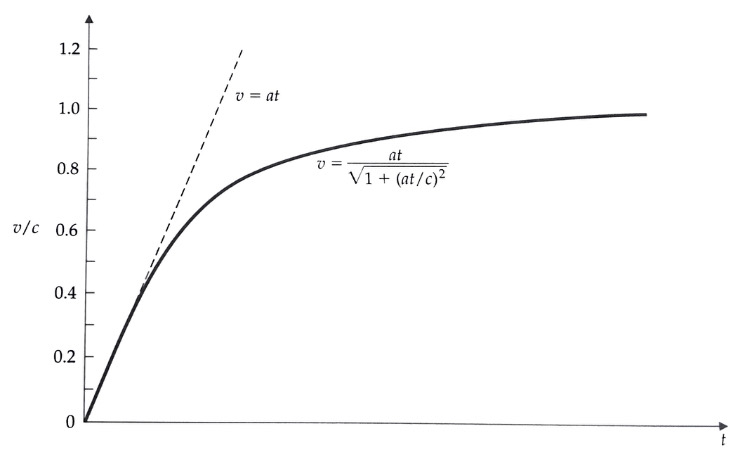
\includegraphics[width=\columnwidth]{constantforce}
\begin{example}
	Find the position of an object of mass $ m $ on which the constant force acts as a function of time. \\
	If we integrate
	\[ u = \dfrac{(F_0t/m)}{\sqrt{1 + \dfrac{F_0^2t^2}{m^2c^2}}} \]
	with respect to time, we will get position. Lets say $ x,t = 0 $ we get
	\[ x ( t ) = \frac { m c ^ { 2 } } { F _ { 0 } } \left( \sqrt { 1 + \frac { F _ { 0 } ^ { 2 } t ^ { 2 } } { m ^ { 2 } c ^ { 2 } } } - 1 \right) \]
	
\end{example}






   	%\chapter{Waves As Particles and Particles As }
\putpic{ch4}
\section{Nature of Photons}
Particles that make up radiation are called photons. \\
Photons travel in the speed of light, as a quanta. The energy is given by
\[ E = pc \]
Energy is also related to the frequency
\[ E = hf \]
where $ h $ is 
\[ h \approx \scinot{6.63}{-34} \mbox{J$ \cdot $ s} \]
Combining the equations we get
\[ p = \frac { E } { c } = \frac { h f } { c } = \frac { h } { \lambda } \]
we can also express it with angular frequency where \[ \omega = 2 \pi f \]
so
\[ E = \hbar \omega \]
where
\[ \hbar = h / 2 \pi \approx 1.05 \times 10 ^ { - 34 } \mathrm { J } \cdot \mathrm { s } \]
is what is usually called Planck's constant. 
\begin{example}
	Suppose that a $ 60 $W bulb radiates light primarily of wavelength $ 1000 $nm. Find the number of photons emitted per second. \\
	We can divide the total energy release per second, Watts, by the energy per photon, to find photons per second.
	\[ n = \frac { 60 \mathrm { W } } { h f } = \frac { 60 \mathrm { W } } { \left( 6.63 \times 10 ^ { - 34 } \mathrm { J } \cdot \mathrm { s } \right) \left( 3 \times 10 ^ { 14 } \mathrm { s } ^ { - 1 } \right) } \]
	$ n  = 3 \times 10 ^ { 20 } \mathrm { photons } / \mathrm { s }$
\end{example}
\section{Photoelectric Effect}
Metals contain a large number of free electrons (sea of electrons).The electrons don't leak but when a photon strikes one of the free electrons the photon may under the right circumstance trigger the electron to escape the metal. \\
Electrons emitted by a metal are called \textbf{photoelectrons}. The \textbf{work function} $ W $ of the metal tells the values for which there will be a current. \\
if $ hf $ is larger than $ W $, then the electrons will emerge with speed $ v $ such that
\[ \dfrac{1}{2} m_e v^2 = hf -W \]
The $ KE $ of an electron is independent of intensity. 
\begin{example}
	EM radiation of wavelength $ 270 \mathrm{ nm } $ on aluminum releases photoelectrons. The most energetic of which are stopped by a potential difference of $ 0.406 $ volts. Calculate work function of aluminum in electron volts. \\
	The energy can be found for the electron using
	\[ K = e V = \left( 1.6 \times 10 ^ { - 19 } \mathrm { C } \right) ( 0.406 \mathrm { V } ) \] \[ = 0.65 \times 10 ^ { - 10 } \mathrm { J } \]
	energy for the photon
	\[ E = h f = \frac { h c } { \lambda } = \] \[ \left( 6.63 \times 10 ^ { - 4 } \mathrm { J } \cdot \mathrm { s } \right) \left( 3.00 \times 10 ^ { 8 } \mathrm { m } / \mathrm { s } \right)\] \[ / \left( 270 \times 10 ^ { - 9 } \mathrm { m } \right) = 737 \times 10 ^ { - 19 } \mathrm { J } \]
	the difference is the work function
	\[ W = E - K = 6.72 \times 10 ^ { - 19 } \mathrm { J }\] \[ = \left( 6.72 \times 10 ^ { - 19 } \mathrm { J } \right) / \left( 1.6 \times 10 ^ { - 19 } \mathrm { J } / \mathrm { eV } \right) = 42 \mathrm { eV } \]
\end{example}
\section{The Compton Effect}
Consider collisions between light and free electrons. That is, 
\[ \gamma + e \rightarrow \gamma + e \]
Let the initial electron be at rest with zero momentum and energy 
\[ m_ec^2 \]
Initially, the photon has energy
\[ hf \]
associated with it is a momentum $ \vec{ \mathrm { q } } $ whose initial magnitude is 
\[ | \vec{ \mathrm { q } }| = hf/c \]
After the collision the photon's energy is $ hf' $ and momentum is $ \vec{ \mathrm { q } }' $.\\
The final electron momentum is \[ \vec{ \mathrm { p } } \] and its energy is 
\[ \sqrt { p ^ { 2 } c ^ { 2 } + m _ { e } ^ { 2 } c ^ { 4 } } \]
conservation of momentum gives us
\[ \vec { q } = \vec { q } ^ { \prime } + \vec { p } \]
and
\[ h f + m _ { e } c ^ { 2 } = h f ^ { \prime } + \sqrt { p ^ { 2 } c ^ { 2 } + m _ { e } ^ { 2 } c ^ { 4 } } \]
So the obvious question is, now what does the light \textit{look} like: what's is wavelength $ \lambda' $?\\
First we see
\[ \begin{aligned} p ^ { 2 } & = \left( \vec { q } ^ { \prime } - \vec { q } \right) ^ { 2 } = q ^ { \prime 2 } + q ^ { 2 } - 2 \vec { q } ^ { \prime } \cdot \vec { q } \\ & = \left( \frac { h f ^ { \prime } } { c } \right) ^ { 2 } + \left( \frac { h f } { c } \right) ^ { 2 } - 2 \left( \frac { h f ^ { \prime } } { c } \right) \left( \frac { h f } { c } \right) \cos \theta \end{aligned} \]
where $ \theta $ is the angle between the initial and final photon momentum vectors. After rearranging we find 
\[ \begin{aligned} p ^ { 2 } + m _ { e } ^ { 2 } c ^ { 2 } & = \left( \frac { h f } { c } - \frac { h f ^ { \prime } } { c } + m _ { s } c \right) ^ { 2 } \\ & = \left( \frac { h f } { c } \right) ^ { 2 } + \left( \frac { h f ^ { \prime } } { c } \right) ^ { 2 } - 2 \left( \frac { h f } { c } \right) \left( \frac { h f ^ { \prime } } { c } \right) \\ & + 2 m _ { e } h \left( f - f ^ { \prime } \right) + m _ { e } ^ { 2 } c ^ { 2 } \end{aligned} \]
substituting in values for $ p^2 $
\[ 2 \left( \frac { h f } { c } \right) \left( \frac { h f ^ { \prime } } { c } \right) ( 1 - \cos \theta ) = 2 m _ { e } h c \left( \frac { f } { c } - \frac { f ^ { \prime } } { c } \right) \]
By using the general relation $ f = c/\lambda $, we easily find that
\[\lambda ^ { \prime } - \lambda = \frac { h } { m _ { e } c } ( 1 - \cos \theta )  \]
This expression tells the \textit{change} $ \Delta \lambda $ after scattering. \\
The parameter 
\[ \frac { h } { m _ { e } c } \]
obviously results in the dimension of length and is called the \textbf{Compton wavelength of the electron}. It's magnitude is
\[ \scinotu{2.4}{-12}{m} \]
\begin{example}
	X ray of $ \lambda = \scinotu{5.53}{-2}{nm} $ is scatter and detected at an angle of $ 35^ \circ $. Find the fractional shift of the wavelength. \\
	\small
	\[ \begin{aligned} \frac { \lambda ^ { \prime } - \lambda } { \lambda } = \frac { h } { m _ { e } c \lambda } ( 1 - \cos \theta ) \\  = \frac { \left( 6.63 \times 10 ^ { - 34 } \mathrm { J } \cdot \mathrm { s } \right) \left( 1 - \cos \left( 35 ^ { \circ } \right) \right) } { \left( 0.91 \times 10 ^ { - 30 } \mathrm { kg } \right) \left( 3.00 \times 10 ^ { 8 } \mathrm { m } / \mathrm { s } \right) \left( 5.53 \times 10 ^ { - 11 } \mathrm { m } \right) } \\ = 7.9 \times 10 ^ { - 3 } \text { . } \end{aligned} \]
	\normalfont
	around a $ 1\% $ shift 
\end{example}
\section{Blackbody Radiation}
What is a blackbody radiation?\\
Black-body radiation is the thermal electromagnetic radiation within or surrounding a body in thermodynamic equilibrium with its environment, or emitted by a black body
Okay...what's a blackbody then?\\
blackbody is an idealized physical body that absorbs all incident electromagnetic radiation, regardless of frequency or angle of incidence. \\
Cool.\\
The blackbody spectrum roughly peaks at 
\[ f _ { \operatorname { man } } = ( 28 ) \frac { k T } { h } = \left( 5.9 \times 10 ^ { 10 } / \mathrm { K } \cdot \mathrm { s } \right) T \]
a result known as \textbf{\textit{Wein displacement law}}.\\
There is also a maximum $ \lambda_{max} $ (Note: that $ \lambda_{max} \neq c/f_{max} $)
\[ \lambda _ { \max } T = 2.9 \times 10 ^ { - 3 } \mathrm { m } \cdot \mathrm { K } \]
\indent This presence of such a maximum gives the prominent color to the radiation of a blackbody. For example, the Sun's surface is at some $ 6000 $K. The maximum wavelength is about $ 480 $nm, the middle range of the human eye, Coincident?! I think not! It actually is not. 
\section{Consequence of Particles as Waves}
Everything is basically a wave. You can use 
\[ \lambda = \dfrac{h}{p} \]
for anything, like dust particles, Ferraro, and ice cream. 
\section{The Nature of Photons+}
In the case of massless particles, like photons, energy is related as
\[ E = |\vec{p}| c \] 
We also know that Energy is related by Planck's constant and frequency
\[ E = hf \]
If we define angular frequency as $ \omega = 2 \pi f $ then we can also get energy as
\[ E = \hbar \omega \]
where \[ \hbar = h/2 \pi \]
\begin{example}
	Suppose that a 60 W lightbulb radiates primarily at a wavelength of 1000 nm, find the photons emitted per second. \\
	We use that 
	\[ f = c/\lambda \approx \scinot{3}{14} Hz \]
	so we can employ
	\begin{align*}
	n = \frac { 60 \mathrm { W } } { h f } = \frac { 60 \mathrm { W } } { \left( 6.63 \times 10 ^ { - 34 } \mathrm { J } \cdot \mathrm { s } \right) \left( 3 \times 10 ^ { 14 } \mathrm { s } ^ { - 1 } \right) } \\
	= 3 \times 10 ^ { 20 } \mathrm { photons/s }
	\end{align*}
\end{example}
\section{The Photoelectric Effect+}
If you strike a metal with a photon at a certain frequency (energy) then it will release electrons. done. \\
This is given by 
\[ \frac{1}{2} m_e v^2 = hf - W \]
where $ W $ is the work function of the metal. 
\begin{example}
	An experiment shows that wen EM radiation of $ \lambda 270$nm falls on an alunium surface, photoelectrons are emitted. The most energetic of these are stopped by a potential difference of $ 0.406 $V. Use this information to calculate the work function of alumninum in electron volts. \\
	The kinetic energy can be found as such
	\begin{align*}
	\begin{array} { c } { K = e V = \left( 1.6 \times 10 ^ { - 19 } \mathrm { C } \right) ( 0.406 \mathrm { V } ) = 0.65 \times 10 ^ { - 19 } \mathrm { J } } \\ { \text { The photon energy is } } \\ { E = h f = \frac { h c } { \lambda } = \left( 6.63 \times 10 ^ { - 34 } \mathrm { J } \cdot \mathrm { s } \right) \left( 3.00 \times 10 ^ { 8 } \mathrm { m } / \mathrm { s } \right) / \left( 270 \times 10 ^ { - 9 } \mathrm { m } \right) = 7.37 \times 10 ^ { - 19 } \mathrm { J } } \\ { \text { The difference is the work function: } } \\ { W = E - K = 6.72 \times 10 ^ { - 19 } \mathrm { J } = \left( 6.72 \times 10 ^ { - 19 } \mathrm { J } \right) / \left( 1.6 \times 10 ^ { - 19 } \mathrm { J } / \mathrm { eV } \right) = 4.2 \mathrm { eV } } 
	\end{array}
	\end{align*} 
\end{example}

\section{The Compton Effect+}
When a photon strikes a stationary electron then the photon and the electron are scattered and the transfer of energy result in a wavelength shift for the photon, which can be detected. 
\putpic{compton}
\\
We can solve for these values. Consider $ \textbf{q} $ the momentum of the photon before it strikes the electron. $ \textbf{q'} $ after it strike. And $ \textbf{p} $ momentum of the electron after being striked
\[ \textbf{q} = \textbf{q'} + \textbf{p} \]
and
\[ hf = m_ec^2 = hf' + \sqrt{p^2c^2 + m_e^2c^4} \]
solving for $ f $ and then $ \lambda $ we find that 
\[ \lambda' - \lambda = \frac{h}{m_2c}(1- \cos \theta) \]
































   	%\chapter{}



























   	%\chapter{}
   	%\chapter{The Schr\"{o}dinger Equation}
\putpic{complex_conjugate}
\section{Wave Functions and Probabilities}
The core understanding arises in 
\[ |\psi(\vec{r}, t)|^2 d^3 \vec{r} \]
The probability of finding an electron in some space. \\
We know that 
\[ \int \limits_{all space} |\psi(\vec{r}, t)|^2 d^3 \vec{r}  = 1 \]
This means that in all of space the probability of finding the electron is guaranteed, which is expected. Sometimes the wave function is not cleanly 1, in which case we normalize it. \\
Based on the relationship between the wave function and its derivative we expect an equation of type the wave function $ \wave $ has to follow the linear relation with it's derivative
\[ \frac{d \wave}{dt} = [some constant] \wave \]
So we can expect it to be the form of some exponential.
\section{The Form of Schrodinger Equation}

We expect some sort of wave function since the particle exhibits wavelike features. This is usually a sine or cosine function, or a combination which we can conveniently express as an exponential. 
\[ \wave = A [ \cos(kx - \omega t) + i \sin(kx - \omega t) ] \]
We can represent this as
\[ \wave = A\exp(i[kx - \omega t]) \]
Where $ k = \dfrac{\lambda}{2 \pi} = \dfrac{h}{2 \pi p} = \dfrac{\hbar}{p}$ and $ \omega = 2 \pi f $ which using $ E = hf $ gives $ \omega = \dfrac{2 \pi E}{h} = \dfrac{E}{\hbar} $
We then find that expecting a plane wave function gives us 
\[ \wave = \exp(i\frac{px-Et}{\hbar}) \]
Taking the first derivative with respect to time and the second derivative with respect to $ x $ we find
\[ \dif{\wave}{t} =  \frac{-iE}{\hbar} \wave\]
\[ \diff{\wave}{x}{2} = \frac{p^2}{h^2} \wave\]
Using $ E = p^2/2m $ for a free particle we can relate the two functions and get the Time Dependent Schrodinger equation
\[ i\hbar \dif{\wave}{t} = -\frac{h^2}{2m} \diff{}{x}{2} \wave \]
If we consider some potential $ V(x) = V_0 $, that will be a part of the energy giving us the complete equation
\[ i\hbar \dif{\wave}{t} = -\frac{h^2}{2m} \diff{}{x}{2} \wave + V(x)\wave\]

\section{Expectations Value}
Normalization. If the value of the integral is not equal to one then the coefficient has to be normalized to agree with this. For certain equations this is very difficult. \\
For convenience the second part of the Schrodinger Equation is called the Hamiltonian. The Hamiltonian is the the operator that only deals with the position part of the Schrodinger equation, and describes the position of the wave function. 
$$ H = -\frac{\hbar^2}{2m} \diff{}{x}{2}  + V(x) $$
The equation can now be rewritten as 
\[ i\hbar \dif{\wave}{t} = H \wave \]
\section{The Time-Independent Schrodinger Equation}
We can use Separation of Variables to separate the wave function $ \wave $. We will use a function for just position $ u(x)  $ and one for just time $ T(t) $. \\
We begin with the Time-Independent Schrodinger equation and use a technique called separation of variables for $ \wave $ to express it as a function of just $ x $. \\
We express the wave function as
\[ \wave = u(x)T(t) \]
Then we use this form in the Schrodinger equation
\[ i\hbar \dif{\wave}{t} = -\frac{\hbar^2}{2m} \diff{}{x}{2} \wave \]
We then find
\[ i\hbar \dif{T(t)}{t} u(x) = -\frac{\hbar^2}{2m} \diff{u(x)}{x}{2} T(t)\]
We can rearrange it as
\[ i\hbar \dif{T(t)}{t} \frac{1}{T(t)} = -\frac{1}{u(x)}\frac{\hbar^2}{2m} \diff{u(x)}{x}{2} \]
Notice that each side of the equation sign is dependent on only $ x $ or $ t $. This means that both sides have to be equal no matter the value of $ x $ or $ t $. Which means that both sides must be a constant, represented by $ E $. So, 
\[ i\hbar \dif{T(t)}{t} \frac{1}{T(t)} = -\frac{1}{u(x)}\frac{\hbar^2}{2m} \diff{u(x)}{x}{2} = E\]
So the Time-Independent Schrodinger equation is 
\[ Eu(x) =  -\frac{\hbar^2}{2m} \diff{u(x)}{x}{2}\]
or
\[ Eu_E(x) = Hu_E(x) \]
We complete this by solving for $ T(t) $ which is 
\[ \dif{T(t)}{t} = \frac{-i E}{\hbar} T(t) \]
So, $ T(t) $ must be
\[ T(t) = \exp(\frac{-iEt}{\hbar}) \]
giving us the wave function as
\[ \wave = u_E(x) \exp(\frac{-iEt}{\hbar}) \]
The solution of $ u_E(x) $ has a special property in that it is the eigenfunction of the operator H, and E is corresponding eigenvalue of that operator. When the eigenfunctions are solved for H, one will find the Bohr's atomic energy levels. 
\section{The Schrodinger Equation in Three Dimensions}
	Deriving in Three Dimensions is not that difficult but with basic understanding of gradient we can get that it is 
\[ i \hbar \dif{\psi(\vec{r}, t)}{t} = -\frac{\hbar^2}{2m} \nabla^2 \cdot \psi(\vec{r}, t) + V(\vec{r}) \cdot \psi(\vec{r}, t) \]
\section{Chapter 6 Problems}
	\begin{q}
	Express the wave function as an integral of finding a particle in all of space.
\end{q}
\begin{q}
	State the expected form of Schrodinger's equation.
\end{q}
\begin{q}
	Derive the time independent Schrodinger Equation
\end{q}
\begin{q}
	What is the Hamiltonian
\end{q}
\begin{q}
	Arrive at the expression of momentum as an operator
\end{q}
\begin{q}
	Derive the time independent Schrodinger Equation
\end{q}
\begin{q}
	State Schrodinger's equation in Three Dimensions
\end{q}
\begin{q}
	Use the time dependent Schrodinger's equation to express the wave function as a second order differential equation of the form 
	\[ f'' + x^2f = 0 \]
\end{q}
\section{Chapter 6 Solutions}
	\begin{ans}
	Probability of finding a particle in ALL of space is obviously one. 
	\[ \int\limits_{all space} | \psi(x,t) | ^2 d^3\vec{r}= 1 \]
\end{ans}
\begin{ans}
	The wave function $ \wave $ has to follow the linear relation with it's derivative
	\[ \frac{d \wave}{dt} = [some constant] \wave \]
	So we can expect it to be the form of some exponential. 
\end{ans}
\begin{ans}
	Based on our expectation of the form of the equation, the wave function is
	\[ \wave = \exp(kx - \omega t) \]
	Where $ k = \dfrac{\lambda}{2 \pi} = \dfrac{h}{2 \pi p} = \dfrac{\hbar}{p}$ and $ \omega = 2 \pi f $ which using $ E = hf $ gives $ \omega = \dfrac{2 \pi E}{h} = \dfrac{E}{\hbar} $
	We then find that expecting a plane wave function gives us 
	\[ \wave = \exp(i\frac{px-Et}{\hbar}) \]
	Taking the first derivative with respect to time and the second derivative with respect to $ x $ we find
	\[ \dif{\wave}{t} =  \frac{-iE}{\hbar} \wave\]
	\[ \diff{\wave}{x}{2} = \frac{p^2}{h^2} \wave\]
	Using $ E = p^2/2m $ for a free particle we can relate the two functions and get the Time Dependent Schrodinger equation
	\[ i\hbar \dif{\wave}{t} = -\frac{h^2}{2m} \diff{}{x}{2} \wave \]
	If we consider some potential $ V(x) = V_0 $, that will be a part of the energy giving us the complete equation
	\[ i\hbar \dif{\wave}{t} = -\frac{h^2}{2m} \diff{}{x}{2} \wave + V(x)\wave\]
\end{ans}
\begin{ans}
	The Hamiltonian is the the operator that only deals with the position part of the Schrodinger equation, and describes the position of the wave function. 
	$$ H = -\frac{\hbar^2}{2m} \diff{}{x}{2}  + V(x) $$
\end{ans}
\begin{ans}
	From the calculation in Problem 3 we can show that
	\[ -i \hbar \dif{}{x} \wave = p \wave \]
	\[ p = -i\hbar \dif{}{x} \]
\end{ans}
\begin{ans}
	We begin with the Time-Independent Schrodinger equation and use a technique called separation of variables for $ \wave $ to express it as a function of just $ x $. \\
	We express the wave function as
	\[ \wave = u(x)T(t) \]
	Then we use this form in the Schrodinger equation
	\[ i\hbar \dif{\wave}{t} = -\frac{\hbar^2}{2m} \diff{}{x}{2} \wave \]
	We then find
	\[ i\hbar \dif{T(t)}{t} u(x) = -\frac{\hbar^2}{2m} \diff{u(x)}{x}{2} T(t)\]
	We can rearrange it as
	\[ i\hbar \dif{T(t)}{t} \frac{1}{T(t)} = -\frac{1}{u(x)}\frac{\hbar^2}{2m} \diff{u(x)}{x}{2} \]
	Notice that each side of the equation sign is dependent on only $ x $ or $ t $. This means that both sides have to be equal no matter the value of $ x $ or $ t $. Which means that both sides must be a constant, represented by $ E $. So, 
	\[ i\hbar \dif{T(t)}{t} \frac{1}{T(t)} = -\frac{1}{u(x)}\frac{\hbar^2}{2m} \diff{u(x)}{x}{2} = E\]
	So the Time-Independent Schrodinger equation is 
	\[ Eu(x) =  -\frac{\hbar^2}{2m} \diff{u(x)}{x}{2}\]
	or
	\[ Eu(x) = Hu(x) \]
	We complete this by solving for $ T(t) $ which is 
	\[ \dif{T(t)}{t} = \frac{-i E}{\hbar} T(t) \]
	So, $ T(t) $ must be
	\[ T(t) = \exp(\frac{-iEt}{\hbar}) \]
	giving us the wave function as
	\[ \wave = u_E(x) \exp(\frac{-iEt}{\hbar}) \]
\end{ans}
\begin{ans}
	Deriving in Three Dimensions is not that difficult but with basic understanding of gradient we can get that it is 
	\[ i \hbar \dif{\psi(\vec{r}, t)}{t} = -\frac{\hbar^2}{2m} \nabla^2 \cdot \psi(\vec{r}, t) + V(\vec{r}) \cdot \psi(\vec{r}, t) \]
\end{ans}
\begin{ans}
	The Time-Independent Schrodinger Equation gives 
	\[ Eu(x) = -\frac{\hbar^2}{2m} \diff{u(x)}{x}{2}\]
	Which we can express in the form
	\[ f'' + \omega^2 f = 0 \]
	So, we find
	\[ \diff{u(x)}{x}{2} + \frac{p^2}{\hbar^2} u(x) = 0  \]
	Giving us
	\[ \omega = \pm \frac{p}{\hbar} \]
\end{ans}
   	%\chapter{Wave Packets and the Uncertainty Principle}
\putpic{uncertainty-principle}
\section{A Free Electron in ONe Dimension}
Schrodinger Equation is
\[ i\hbar \dif{\wave}{t} = -\frac{h^2}{2m} \diff{}{x}{2} \wave + V(x)\wave\]
The time independent form wave equation is 
\[ \wave = u_E(x) \exp(\frac{-iEt}{\hbar}) \]
Since, Schrodinger's equation is a relationship between a function and it's second derivative we can try to express it like a spring function. the wave function as a second order differential equation of the form 
\[ f'' + k^2f = 0 \]
The Time-Independent Schrodinger Equation gives 
\[ Eu(x) = -\frac{\hbar^2}{2m} \diff{u(x)}{x}{2}\]
Which we can express in the form
\[ f'' + k^2 f = 0 \]
So, we find
\[ \diff{u(x)}{x}{2} + \frac{p^2}{\hbar^2} u(x) = 0  \]
Giving us
\[ k = \pm \frac{p}{\hbar} \]
or 
\[ p = \pm \hbar k \]
One important step is to normalize the wave function. That is 
\[ insert \]
\section{Wave Packets}
Solving for the probability distribution for the wave function gives 
\[ \Delta x = 4 \pi \hbar / \Delta p \]
the superposition of plane waves made up of weights that cover a finite range of momenta $ \Delta p $ is known as a wave packet. 
\section{Gaussian Wave Packet}
A wave packet without dispersion (real or imaginary part)
A wave packet with dispersion
In physics, a wave packet (or wave train) is a short "burst" or "envelope" of localized wave action that travels as a unit. 
\section{The Meaning of Uncertainty Relations}
\begin{example}
	Consider a grain of dust of mass $ \scinot{1}{-7} $ moving with a velocity around $ 10 m/s $ suppose that the measuring instrument has a local uncertainty of $ \scinot{1}{-6} m $, Find the intrinsic uncertainty in position. 
	\begin{align*}
	\begin{array} { c } { \Delta p = m \Delta v = \left( 10 ^ { - 7 } \mathrm { kg } \right) \left( 10 ^ { - 6 } \mathrm { m } / \mathrm { s } \right) = 10 ^ { - 13 } \mathrm { kg } \cdot \mathrm { m } / \mathrm { s } } \\ \intertext { Hence, according to the uncertainty relation, the position could at best be measured to within a window}\\ { \Delta x \equiv \frac { \hbar } { \Delta p } = \frac { \left( 1.05 \times 10 ^ { - 34 } \mathrm { J } \cdot \mathrm { s } \right) } { \left( 10 ^ { - 13 } \mathrm { kg } \cdot \mathrm { m } / \mathrm { s } \right) } \equiv 10 ^ { - 21 } \mathrm { m } } \end{array}
	\end{align*}
\end{example}
\section{The Time Energy Uncertainty Relation}
An extension of the previous uncertainty principle is time and energy. \\
\begin{align}
\begin{array} { c } { \Delta E = v \Delta p \geq v \frac { \hbar / 2 } { \Delta x } = \frac { \hbar / 2 } { ( \Delta x / v ) } = \frac { \hbar / 2 } { \Delta t } } \\ { \Delta E \Delta t \geq \hbar / 2 } \end{array}
\end{align}
Consider the case where the time interval is so short that the energy can be low enough to dissassociate and then come back together. 
   	%
\chapter{Barriers and Wells}
	Classically, we expect that when a particle with fixed momentum and energy approaches a potential barrier then it will get either reflected or transmitted. In quantum mechanics, we see that this does not actually happen and a certain amount will get transmitted and reflected. This should be a little more obvious considering that we understand the particles are a wave as well, so in this case since the wavelength is so much larger we can expect it to behave like this around the potential barrier. \\
An interesting consequence is tunneling, when a particle goes through the potential barrier.
\section{Particle Motion in the Presence of a Potential Barrier}
A one-dimensional potential barrier is formed by a potential-energy function of the form
\[ V(x) = \begin{cases}
0 \text{ for } x < -a \\
V_0 \text{ for } -a < x < a \\
0 \text{ for } x > +a 
\end{cases} \]
\putpic{bar}
We basically have to cases arise. \\
If $ E > V_0 $ then the particle will pass trough the barrier, but as the particle passes through we realize that the energy is reduced. Initially, the energy of the particle is given by 
\[ E = \frac{p^2}{2m} \] but with the potential barrier we have \[ E = \frac{p^2}{2m} + V_0\]
Solving for the momentum we find that it is reduced to 
\[ p = \sqrt{2m(E-V_0)} \]
If $ E < V_0 $ then the particle hits a wall and is reflected back to the left. 
\putpic{tunel}
\section{Wave Functions in the Presence of a Potential Barrier}
We can see how what is described qualitatively is realized through solving Schrodinger's equation. \\
With the notation
\[ k = p/\hbar \]
In region I the Schrodinger equation is
\[ \diff{u(x)}{x}{2} + \frac{2m}{\hbar ^2} E u(x) = 0 \]
where $ E = \hbar^2k^2/2m $. We expect that in region I, because of the presence of the potential, we will have a wave function that represent the incoming wave and a possible reflected wave. This wave function will have the same time independent factor
\[ \exp(-iEt/\hbar) \]
which we can drop. Thus we have\\
Region I
\[ u(x) = \exp(ikx) + R \exp(-ikx) \]
For region II the Schrodinger equation is
\[ \diff{u(x)}{x}{2} + \frac{2m}{\hbar ^2} (E-V_0) u(x) = 0 \]
The second part is negative because of the negative momentum. Simply, $ R $ is how much of the incident wave is reflected. \\
instead of $ k $ we use $ q $ where
\[ q^2 = \frac{2m}{\hbar^2} (E - V_0)\]
For $ q $ we will get a $ \pm $ so we have two coefficients accordingly for that
\[ u(x) = A \exp (iqx) + B \exp(-iqx) \]
In Region III, the only part of the wave that's coming out is the transmitted part so we know the equation will be 
\[ u(x) = T \exp (iqx)  \]
To solve for the coefficients the one restriction we have is that we expect the probability distribution to be continuous, so we set the restriction that the first derivative must be continuous everywhere. Since, the equation was formed from the function and its second derivative this is a reasonable expectation. 
\begin{example}
	Solve for $ R $ and $ T $ \\
	\begin{align}
	\begin{array} { c } { R = \frac { i \left( q ^ { 2 } - k ^ { 2 } \right) \sin ( 2 q a ) } { 2 k q \cos ( 2 q a ) - i \left( k ^ { 2 } + q ^ { 2 } \right) \sin ( 2 q a ) } \exp ( - 2 i k a ) } \\ { T = \frac { 2 k q } { 2 k q \cos ( 2 q a ) - i \left( k ^ { 2 } + q ^ { 2 } \right) \sin ( 2 q a ) } \exp ( - 2 i k a ) } \end{array}
	\end{align}
	The interesting point is that even for $ E > V_0 $ the above equations do no equal zero. 
\end{example}
\begin{example}
	\putpic{step}
	Consider a beam of electrons traveling to the right along the $ x $-axis with energy $ E $. The potential energy is $ V = 0 $ for $ x < 0 $ but at $ x = 0 $ there is a potential "step" and the potential energy increases to (positive) $ V_0 $ for $ x > 0 $ Assuming that $ E > V_0 $ calculate the reflection and transmission coeffients, and show the flux is conserved. \\
	We basically have at the point $ x = 0 $
	\[ u(x) = \exp(ikx) + R \exp(-ikx) \]
	and
	\[ u(x) = T \exp(iqx) \]
	Taking the derivative of each reveals 
	\[ \dif{u(x)}{x} = ik\exp(ikx) - ikR \exp(-ikx) \]
	\[ \dif{u(x)}{x} = ik T \exp(iqx) \]
	For the value of $ x = 0 $ we get 
	\begin{align*}
	u(0) &= 1 + R \\
	&= T \\
	\intertext{and}
	\dif{u(0)}{x} &= ik - ikR \\
	&= iqT
	\end{align*}
	Leaving us with two equations
	\[ T = 1 + R \]
	\[ k - kR = qT \]
	We can rearrange the second one and get
	\begin{align*}
	\frac{k}{q} (1 - R) = T = 1 +R \\
	k - Rk = q + Rq \\
	\frac{k-q}{k+q} = R \\
	\frac{2k}{k+q} = T
	\end{align*}
\end{example}

\section{Tunneling through the Potential Barrier}
 Suppose that the incoming energy $ E < V_0 $. So, 
 \[ q^2 = \frac{2m}{\hbar^2} (E-V_0) < 0 \]
 Obviously $ q $ is complex. So, we rewrite it as 
 \[ q \rightarrow i \kappa \]
 \[ \kappa^2 = \frac{2m}{\hbar^2} (V_0 - E) \]
We can then just plug in the other form of $ q $ and adjust our solutions for the coefficients. 
\begin{example}
	Consider a $ 2000 $kg truck moving towards a bump in the road whose center is at $ x = 0 $ and whose height is given by $ 0 $ for $ x<-0.1 $m, $ (0.05m)\cos(5 \pi x)  $ for $ -0.1m < x < +0.1m $. Assuming that the truck moves so slowly that its kinetic energy is insufficient to climb the bump to any height at all, estimate the probability for the truck to tunnel through the bump. \\
	The probability transmission is only dependent on $ |T|^2 $ so we have 
	\begin{align*}
	\begin{aligned} | T | ^ { 2 } & \cong \exp \left( - \frac { 2 } { \hbar } \int \sqrt { 2 m V ( x ) } d x \right) \\ & = \exp \left( - \frac { 2 \sqrt { 2 ( 2,000 k g ) ( 2,000 k g ) \left( 9.8 m / s ^ { 2 } \right) ( 0.05 m ) } } { 1.05 \times 10 ^ { - 34 } J \cdot s } \right. \end{aligned}
	\end{align*}
	The remaining integral is then given by
	\begin{align*}
	\frac { 1 } { 5 \pi } [ \sin ( 0.5 \pi ) - \sin ( - 0.5 \pi ) ] = \frac { 2 } { 5 \pi } \cong 0.13
	\end{align*}
	Substituting into the expression for $ |T|^2 $ yields the rest of therms so we get that 
	\[ |T|^2 \approxeq \exp(\scinot{-5}{36}) \]
	Since, Planck's constant is so small for macro scales it is basically zero. 
\section{Bound States}
	We are interested in how the Schrodinger Equation determines the energies of the trapped states that occur in an infinite well. 
\end{example}
\section{Problems 6-8}
\begin{q}
	Express the wave function as an integral of finding a particle in all of space.
\end{q}
\begin{q}
	State the expected form of Schrodinger's equation.
\end{q}
\begin{q}
	Derive the time independent Schrodinger Equation
\end{q}
\begin{q}
	What is the Hamiltonian
\end{q}
\begin{q}
	Arrive at the expression of momentum as an operator
\end{q}
\begin{q}
	Derive the time independent Schrodinger Equation
\end{q}
\begin{q}
	State Schrodinger's equation in Three Dimensions
\end{q}
\begin{q}
	Use the time dependent Schrodinger's equation to express the wave function as a second order differential equation of the form 
	\[ f'' + x^2f = 0 \]
\end{q}
\begin{q}
	State Heisenberg's Uncertainty Relation
\end{q}
\begin{q}
	Arrive at the Time-Energy Uncertainty Relation
\end{q}
\begin{q}
	Wave function at the presence of a barrier. Consider some potential barrier in Region II. Region I is before the potential barrier and Region III is after the potential barrier.\\
	State the Schrodinger Equation in each Region and the form of the wave function.
\end{q}
\begin{q}
	Solve for the reflection and transmission coefficient.
\end{q}
\begin{q}
	Consider a beam of electrons traveling to the right along the $ x$-axis with energy $ E $. The potential energy is $ V = 0 $ for $ x < 0 $, but as $ x = 0 $ there is a potential step, and the potential energy increases to $ V_0 $ for $ x > 0 $. Assuming $ E > V_0 $ (a) calculate the reflection and transmission coefficients, and (b) show that flux is conserved. 
\end{q}
\begin{q}
	Consider a $ 2000 $kg truck moving towards a bump in the road whose center is at $ x = 0 $ and whose height is given by $ 0 $ for $ x<-0.1 $m, $ (0.05m)\cos(5 \pi x)  $ for $ -0.1m < x < +0.1m $. Assuming that the truck moves so slowly that its kinetic energy is insufficient to climb the bump to any height at all, estimate the probability for the truck to tunnel through the bump.
\end{q}
\section{Solutions}
	\begin{ans}
	Probability of finding a particle in ALL of space is obviously one. 
	\[ \int\limits_{all space} | \psi(x,t) | ^2 d^3\vec{r}= 1 \]
\end{ans}
\begin{ans}
	The wave function $ \wave $ has to follow the linear relation with it's derivative
	\[ \frac{d \wave}{dt} = [some constant] \wave \]
	So we can expect it to be the form of some exponential. 
\end{ans}
\begin{ans}
	Based on our expectation of the form of the equation, the wave function is
	\[ \wave = \exp(kx - \omega t) \]
	Where $ k = \dfrac{\lambda}{2 \pi} = \dfrac{h}{2 \pi p} = \dfrac{\hbar}{p}$ and $ \omega = 2 \pi f $ which using $ E = hf $ gives $ \omega = \dfrac{2 \pi E}{h} = \dfrac{E}{\hbar} $
	We then find that expecting a plane wave function gives us 
	\[ \wave = \exp(i\frac{px-Et}{\hbar}) \]
	Taking the first derivative with respect to time and the second derivative with respect to $ x $ we find
	\[ \dif{\wave}{t} =  \frac{-iE}{\hbar} \wave\]
	\[ \diff{\wave}{x}{2} = \frac{p^2}{h^2} \wave\]
	Using $ E = p^2/2m $ for a free particle we can relate the two functions and get the Time Dependent Schrodinger equation
	\[ i\hbar \dif{\wave}{t} = -\frac{h^2}{2m} \diff{}{x}{2} \wave \]
	If we consider some potential $ V(x) = V_0 $, that will be a part of the energy giving us the complete equation
	\[ i\hbar \dif{\wave}{t} = -\frac{h^2}{2m} \diff{}{x}{2} \wave + V(x)\wave\]
\end{ans}
\begin{ans}
	The Hamiltonian is the the operator that only deals with the position part of the Schrodinger equation, and describes the position of the wave function. 
	$$ H = -\frac{\hbar^2}{2m} \diff{}{x}{2}  + V(x) $$
\end{ans}
\begin{ans}
	From the calculation in Problem 3 we can show that
	\[ -i \hbar \dif{}{x} \wave = p \wave \]
	\[ p = -i\hbar \dif{}{x} \]
\end{ans}
\begin{ans}
	We begin with the Time-Independent Schrodinger equation and use a technique called separation of variables for $ \wave $ to express it as a function of just $ x $. \\
	We express the wave function as
	\[ \wave = u(x)T(t) \]
	Then we use this form in the Schrodinger equation
	\[ i\hbar \dif{\wave}{t} = -\frac{\hbar^2}{2m} \diff{}{x}{2} \wave \]
	We then find
	\[ i\hbar \dif{T(t)}{t} u(x) = -\frac{\hbar^2}{2m} \diff{u(x)}{x}{2} T(t)\]
	We can rearrange it as
	\[ i\hbar \dif{T(t)}{t} \frac{1}{T(t)} = -\frac{1}{u(x)}\frac{\hbar^2}{2m} \diff{u(x)}{x}{2} \]
	Notice that each side of the equation sign is dependent on only $ x $ or $ t $. This means that both sides have to be equal no matter the value of $ x $ or $ t $. Which means that both sides must be a constant, represented by $ E $. So, 
	\[ i\hbar \dif{T(t)}{t} \frac{1}{T(t)} = -\frac{1}{u(x)}\frac{\hbar^2}{2m} \diff{u(x)}{x}{2} = E\]
	So the Time-Independent Schrodinger equation is 
	\[ Eu(x) =  -\frac{\hbar^2}{2m} \diff{u(x)}{x}{2}\]
	or
	\[ Eu(x) = Hu(x) \]
	We complete this by solving for $ T(t) $ which is 
	\[ \dif{T(t)}{t} = \frac{-i E}{\hbar} T(t) \]
	So, $ T(t) $ must be
	\[ T(t) = \exp(\frac{-iEt}{\hbar}) \]
	giving us the wave function as
	\[ \wave = u_E(x) \exp(\frac{-iEt}{\hbar}) \]
\end{ans}
\begin{ans}
	Deriving in Three Dimensions is not that difficult but with basic understanding of gradient we can get that it is 
	\[ i \hbar \dif{\psi(\vec{r}, t)}{t} = -\frac{\hbar^2}{2m} \nabla^2 \cdot \psi(\vec{r}, t) + V(\vec{r}) \cdot \psi(\vec{r}, t) \]
\end{ans}
\begin{ans}
	The Time-Independent Schrodinger Equation gives 
	\[ Eu(x) = -\frac{\hbar^2}{2m} \diff{u(x)}{x}{2}\]
	Which we can express in the form
	\[ f'' + \omega^2 f = 0 \]
	So, we find
	\[ \diff{u(x)}{x}{2} + \frac{p^2}{\hbar^2} u(x) = 0  \]
	Giving us
	\[ \omega = \pm \frac{p}{\hbar} \]
\end{ans}
\begin{ans}
	Based on observational results and modifying the Schrodinger Equation we find
	\[ \Delta p \Delta x \leq \dfrac{\hbar}{2} \]
\end{ans}
\begin{ans}
	With some 
	\begin{align}
	\begin{array} { c } { \Delta E = v \Delta p \geq v \frac { \hbar / 2 } { \Delta x } = \frac { \hbar / 2 } { ( \Delta x / v ) } = \frac { \hbar / 2 } { \Delta t } } \\ { \Delta E \Delta t \geq \hbar / 2 } \end{array}
	\end{align}
\end{ans}
\begin{ans}
	Region I:
	A combination of the initial wave and the part being reflected back. 
	From Problem 8 we know that $ \omega = \pm p/\hbar $, so we state that the wave function must be of the form 
	\[ u(x) = exp(ikx) \]
	where 
	\[ k = p/\hbar \]
	So the wave function in region I must be 
	$$ u(x) = \exp(ikx) + R\exp(-ikx) $$
	For region II since there is a potential so we have
	\[ \diff{u(x)}{x}{2} + \frac{(E-V_0) 2m}{\hbar^2} u(x) \]
	We can set $ q $ as 
	\[ q = \pm \sqrt\frac{(E-V_0) 2m}{\hbar^2} \]
	So we have the function as
	\[ u(x) = A \exp (ikx) + B \exp (-ikx) \]
	For region III since the energy is the same as region I, but there is only the wave being transmitted we have 
	\[ u(x) = T \exp(ikx)\]
\end{ans}
\begin{ans}
	\begin{align}
	\begin{array} { c } { R = \frac { i \left( q ^ { 2 } - k ^ { 2 } \right) \sin ( 2 q a ) } { 2 k q \cos ( 2 q a ) - i \left( k ^ { 2 } + q ^ { 2 } \right) \sin ( 2 q a ) } \exp ( - 2 i k a ) } \\ { T = \frac { 2 k q } { 2 k q \cos ( 2 q a ) - i \left( k ^ { 2 } + q ^ { 2 } \right) \sin ( 2 q a ) } \exp ( - 2 i k a ) } \end{array}
	\end{align}
\end{ans}
\begin{ans}
	We basically have at the point $ x = 0 $
	\[ u(x) = \exp(ikx) + R \exp(-ikx) \]
	and
	\[ u(x) = T \exp(iqx) \]
	Taking the derivative of each reveals 
	\[ \dif{u(x)}{x} = ik\exp(ikx) - ikR \exp(-ikx) \]
	\[ \dif{u(x)}{x} = ik T \exp(iqx) \]
	For the value of $ x = 0 $ we get 
	\begin{align*}
	u(0) &= 1 + R \\
	&= T \\
	\intertext{and}
	\dif{u(0)}{x} &= ik - ikR \\
	&= iqT
	\end{align*}
	Leaving us with two equations
	\[ T = 1 + R \]
	\[ k - kR = qT \]
	We can rearrange the second one and get
	\begin{align*}
	\frac{k}{q} (1 - R) = T = 1 +R \\
	k - Rk = q + Rq \\
	\frac{k-q}{k+q} = R \\
	\frac{2k}{k+q} = T
	\end{align*}
\end{ans}
\begin{ans}
	The probability transmission is only dependent on $ |T|^2 $ so we have 
	\begin{align*}
	\begin{aligned} | T | ^ { 2 } & \cong \exp \left( - \frac { 2 } { \hbar } \int \sqrt { 2 m V ( x ) } d x \right) \\ & = \exp \left( - \frac { 2 \sqrt { 2 ( 2,000 k g ) ( 2,000 k g ) \left( 9.8 m / s ^ { 2 } \right) ( 0.05 m ) } } { 1.05 \times 10 ^ { - 34 } J \cdot s } \right. \end{aligned}
	\end{align*}
	The remaining integral is then given by
	\begin{align*}
	\frac { 1 } { 5 \pi } [ \sin ( 0.5 \pi ) - \sin ( - 0.5 \pi ) ] = \frac { 2 } { 5 \pi } \cong 0.13
	\end{align*}
	Substituting into the expression for $ |T|^2 $ yields the rest of therms so we get that 
	\[ |T|^2 \approxeq \exp(\scinot{-5}{36}) \]
	Since, Planck's constant is so small for macro scales it is basically zero. 
\end{ans}


   	%\input{chapter09.tex}
   	%\input{chapter10.tex}
   	%\input{chapter11.tex}
   	%\input{chapter12.tex}
   	%\input{chapter13.tex}
   	%\input{chapter14.tex}
   	%\input{chapter15.tex}
   	%\input{chapter16.tex}
   	%\input{chapter17.tex}
   	%\input{chapter18.tex}
   	
\end{document}